\section{Profiling}
\label{sec:profile}
%Taejoon%
\subsection{Profiling}
In order to find the bottlenecks of path, we first profiled our code
using Intel's VTune Amplifier (It was broken in cluster, so we used
it on local machine), as shown in Figure \ref{amplxe-command}.

\vspace{0.3cm}

\begin{figure}[H]
\footnotesize
\begin{verbatim}
amplxe-cl -collect advanced-hotspots ./path
amplxe-cl -report hotspots -source-object function=<NAME>
\end{verbatim}
\caption{VTune Amplifier Command}
\label{amplxe-command}
\end{figure}

\subsection{Initial Profiling Result}
Initial profile result can be found at Figure \ref{initial_profile_result_0},
and more detail in Figure \ref{initial_profile_result_1}.

We found that "square" function is the main bottleneck and do the most critical
steps for this program, so this point is where we started to tune the code.

\begin{figure}[H]
    \centering
    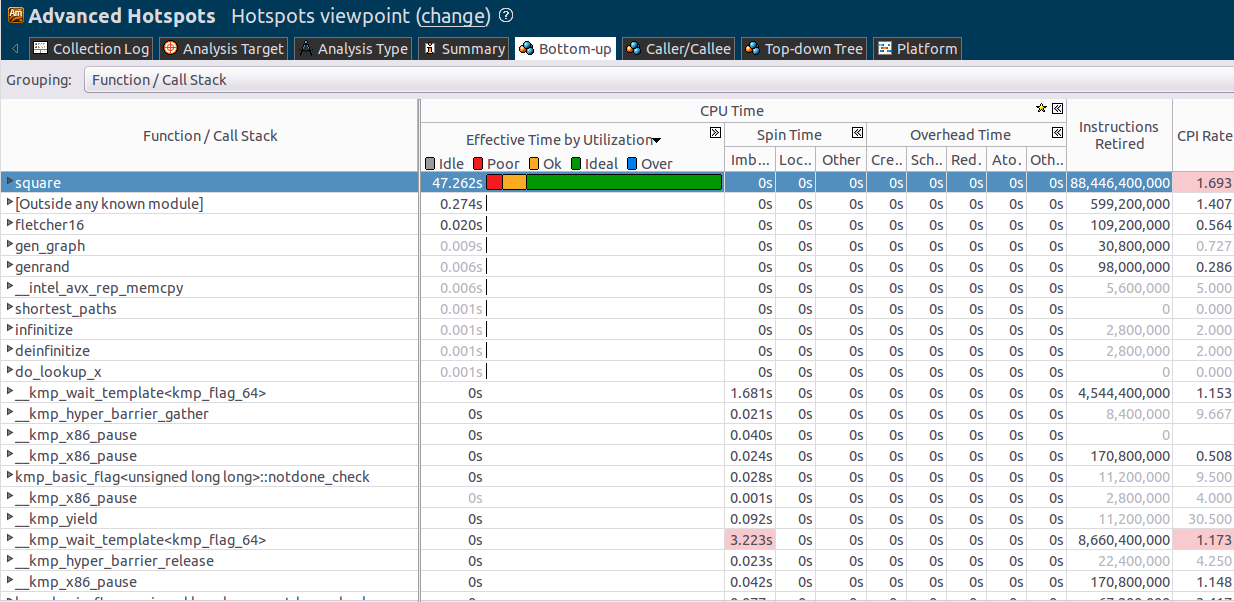
\includegraphics[width=0.65\textwidth]{figs/0_analysis.png}
    \caption{Initial Profile Analysis}
    \label{initial_profile_result_0}
\end{figure}

\begin{figure}[H]
    \centering
    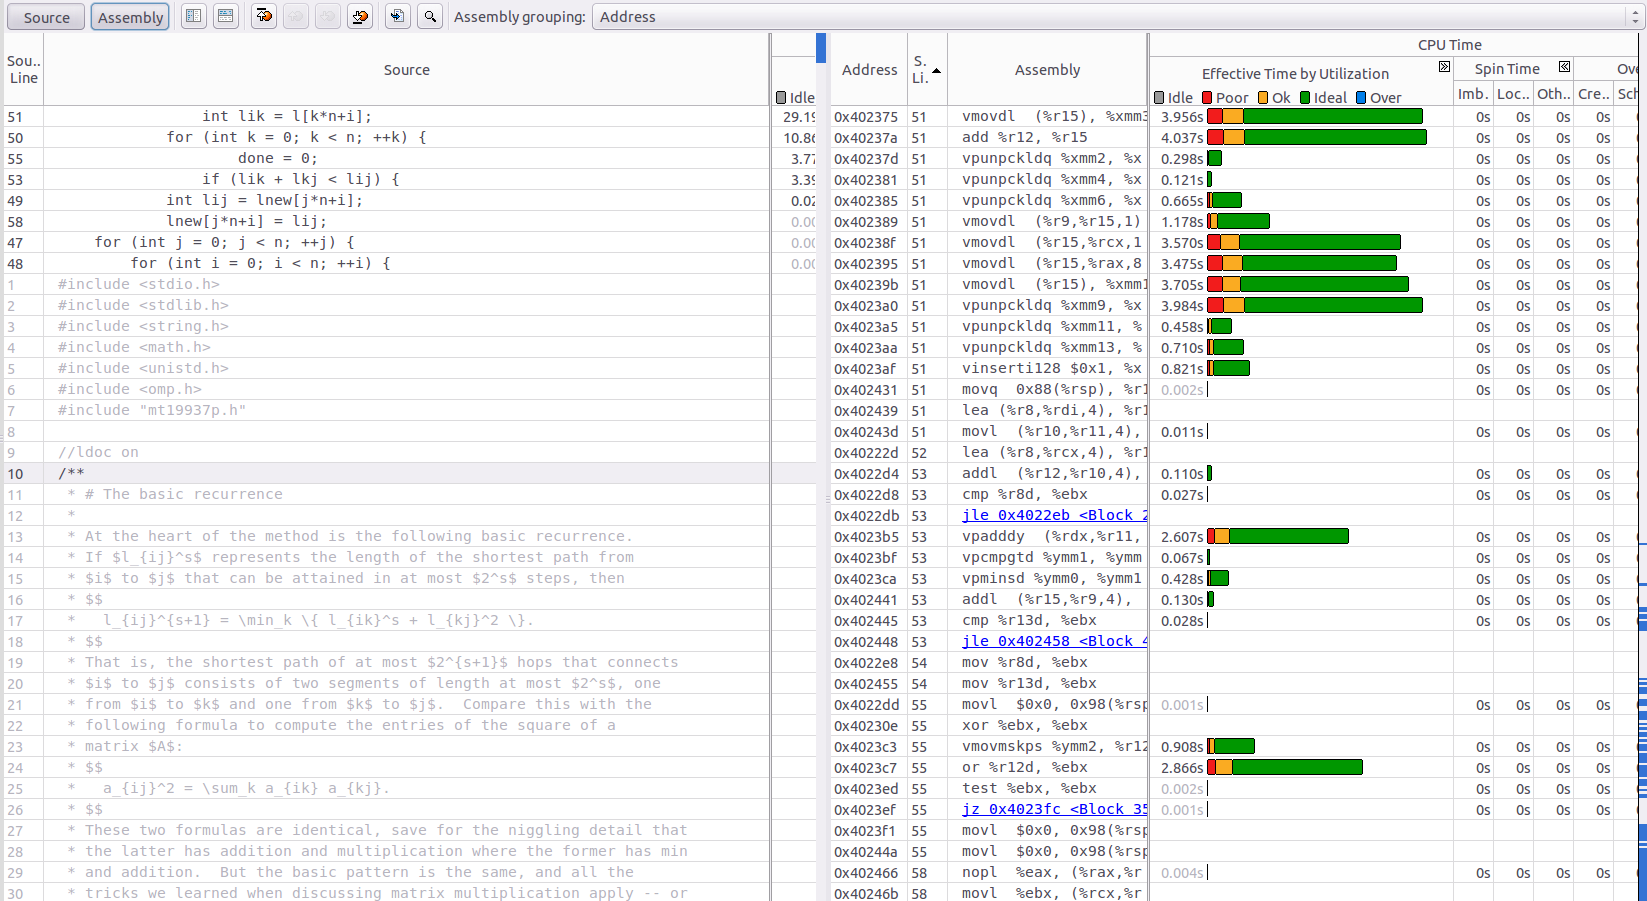
\includegraphics[width=0.65\textwidth]{figs/0_assembly.png}
    \caption{Initial Assembly Result}
    \label{initial_profile_result_1}
\end{figure}

\subsection{Initial Timing Result}

Initial timing result is shown in Figure \ref{initial_profile_result_2}. As we
can see the program is running with 8 threads using OpenMP and it takes 11.0818
seconds for 2000 vertices.

\begin{figure}[H]
    \centering
    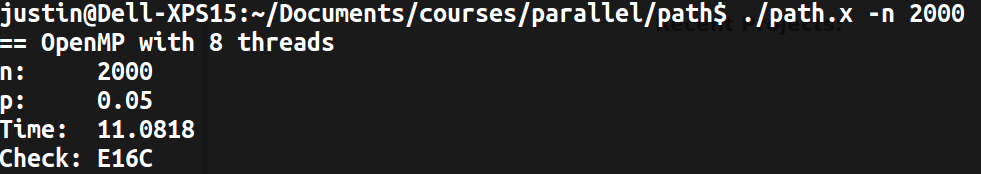
\includegraphics[width=0.8\textwidth]{figs/0_timing.png}
    \caption{Initial Timing Result}
    \label{initial_profile_result_2}
\end{figure}

